\documentclass[]{article}
\usepackage{lmodern}
\usepackage{amssymb,amsmath}
\usepackage{ifxetex,ifluatex}
\usepackage{fixltx2e} % provides \textsubscript
\ifnum 0\ifxetex 1\fi\ifluatex 1\fi=0 % if pdftex
  \usepackage[T1]{fontenc}
  \usepackage[utf8]{inputenc}
\else % if luatex or xelatex
  \ifxetex
    \usepackage{mathspec}
  \else
    \usepackage{fontspec}
  \fi
  \defaultfontfeatures{Ligatures=TeX,Scale=MatchLowercase}
\fi
% use upquote if available, for straight quotes in verbatim environments
\IfFileExists{upquote.sty}{\usepackage{upquote}}{}
% use microtype if available
\IfFileExists{microtype.sty}{%
\usepackage{microtype}
\UseMicrotypeSet[protrusion]{basicmath} % disable protrusion for tt fonts
}{}
\usepackage[margin=1in]{geometry}
\usepackage{hyperref}
\hypersetup{unicode=true,
            pdftitle={Logging using ParallelLogger},
            pdfauthor={Martijn J. Schuemie},
            pdfborder={0 0 0},
            breaklinks=true}
\urlstyle{same}  % don't use monospace font for urls
\usepackage{color}
\usepackage{fancyvrb}
\newcommand{\VerbBar}{|}
\newcommand{\VERB}{\Verb[commandchars=\\\{\}]}
\DefineVerbatimEnvironment{Highlighting}{Verbatim}{commandchars=\\\{\}}
% Add ',fontsize=\small' for more characters per line
\usepackage{framed}
\definecolor{shadecolor}{RGB}{248,248,248}
\newenvironment{Shaded}{\begin{snugshade}}{\end{snugshade}}
\newcommand{\AlertTok}[1]{\textcolor[rgb]{0.94,0.16,0.16}{#1}}
\newcommand{\AnnotationTok}[1]{\textcolor[rgb]{0.56,0.35,0.01}{\textbf{\textit{#1}}}}
\newcommand{\AttributeTok}[1]{\textcolor[rgb]{0.77,0.63,0.00}{#1}}
\newcommand{\BaseNTok}[1]{\textcolor[rgb]{0.00,0.00,0.81}{#1}}
\newcommand{\BuiltInTok}[1]{#1}
\newcommand{\CharTok}[1]{\textcolor[rgb]{0.31,0.60,0.02}{#1}}
\newcommand{\CommentTok}[1]{\textcolor[rgb]{0.56,0.35,0.01}{\textit{#1}}}
\newcommand{\CommentVarTok}[1]{\textcolor[rgb]{0.56,0.35,0.01}{\textbf{\textit{#1}}}}
\newcommand{\ConstantTok}[1]{\textcolor[rgb]{0.00,0.00,0.00}{#1}}
\newcommand{\ControlFlowTok}[1]{\textcolor[rgb]{0.13,0.29,0.53}{\textbf{#1}}}
\newcommand{\DataTypeTok}[1]{\textcolor[rgb]{0.13,0.29,0.53}{#1}}
\newcommand{\DecValTok}[1]{\textcolor[rgb]{0.00,0.00,0.81}{#1}}
\newcommand{\DocumentationTok}[1]{\textcolor[rgb]{0.56,0.35,0.01}{\textbf{\textit{#1}}}}
\newcommand{\ErrorTok}[1]{\textcolor[rgb]{0.64,0.00,0.00}{\textbf{#1}}}
\newcommand{\ExtensionTok}[1]{#1}
\newcommand{\FloatTok}[1]{\textcolor[rgb]{0.00,0.00,0.81}{#1}}
\newcommand{\FunctionTok}[1]{\textcolor[rgb]{0.00,0.00,0.00}{#1}}
\newcommand{\ImportTok}[1]{#1}
\newcommand{\InformationTok}[1]{\textcolor[rgb]{0.56,0.35,0.01}{\textbf{\textit{#1}}}}
\newcommand{\KeywordTok}[1]{\textcolor[rgb]{0.13,0.29,0.53}{\textbf{#1}}}
\newcommand{\NormalTok}[1]{#1}
\newcommand{\OperatorTok}[1]{\textcolor[rgb]{0.81,0.36,0.00}{\textbf{#1}}}
\newcommand{\OtherTok}[1]{\textcolor[rgb]{0.56,0.35,0.01}{#1}}
\newcommand{\PreprocessorTok}[1]{\textcolor[rgb]{0.56,0.35,0.01}{\textit{#1}}}
\newcommand{\RegionMarkerTok}[1]{#1}
\newcommand{\SpecialCharTok}[1]{\textcolor[rgb]{0.00,0.00,0.00}{#1}}
\newcommand{\SpecialStringTok}[1]{\textcolor[rgb]{0.31,0.60,0.02}{#1}}
\newcommand{\StringTok}[1]{\textcolor[rgb]{0.31,0.60,0.02}{#1}}
\newcommand{\VariableTok}[1]{\textcolor[rgb]{0.00,0.00,0.00}{#1}}
\newcommand{\VerbatimStringTok}[1]{\textcolor[rgb]{0.31,0.60,0.02}{#1}}
\newcommand{\WarningTok}[1]{\textcolor[rgb]{0.56,0.35,0.01}{\textbf{\textit{#1}}}}
\usepackage{graphicx,grffile}
\makeatletter
\def\maxwidth{\ifdim\Gin@nat@width>\linewidth\linewidth\else\Gin@nat@width\fi}
\def\maxheight{\ifdim\Gin@nat@height>\textheight\textheight\else\Gin@nat@height\fi}
\makeatother
% Scale images if necessary, so that they will not overflow the page
% margins by default, and it is still possible to overwrite the defaults
% using explicit options in \includegraphics[width, height, ...]{}
\setkeys{Gin}{width=\maxwidth,height=\maxheight,keepaspectratio}
\IfFileExists{parskip.sty}{%
\usepackage{parskip}
}{% else
\setlength{\parindent}{0pt}
\setlength{\parskip}{6pt plus 2pt minus 1pt}
}
\setlength{\emergencystretch}{3em}  % prevent overfull lines
\providecommand{\tightlist}{%
  \setlength{\itemsep}{0pt}\setlength{\parskip}{0pt}}
\setcounter{secnumdepth}{5}
% Redefines (sub)paragraphs to behave more like sections
\ifx\paragraph\undefined\else
\let\oldparagraph\paragraph
\renewcommand{\paragraph}[1]{\oldparagraph{#1}\mbox{}}
\fi
\ifx\subparagraph\undefined\else
\let\oldsubparagraph\subparagraph
\renewcommand{\subparagraph}[1]{\oldsubparagraph{#1}\mbox{}}
\fi

%%% Use protect on footnotes to avoid problems with footnotes in titles
\let\rmarkdownfootnote\footnote%
\def\footnote{\protect\rmarkdownfootnote}

%%% Change title format to be more compact
\usepackage{titling}

% Create subtitle command for use in maketitle
\newcommand{\subtitle}[1]{
  \posttitle{
    \begin{center}\large#1\end{center}
    }
}

\setlength{\droptitle}{-2em}

  \title{Logging using ParallelLogger}
    \pretitle{\vspace{\droptitle}\centering\huge}
  \posttitle{\par}
    \author{Martijn J. Schuemie}
    \preauthor{\centering\large\emph}
  \postauthor{\par}
      \predate{\centering\large\emph}
  \postdate{\par}
    \date{2019-01-18}


\begin{document}
\maketitle

{
\setcounter{tocdepth}{2}
\tableofcontents
}
\hypertarget{introduction}{%
\section{Introduction}\label{introduction}}

This vignette describes how you can use the \texttt{ParallelLogger}
package to perform logging. Logging is the activity of recording events
that occur during an analysis in a log. The log can be used for example
for for debugging, profiling (understanding performance bottlenecks),
and audits.

\hypertarget{terminology}{%
\subsection{Terminology}\label{terminology}}

\begin{itemize}
\tightlist
\item
  \textbf{Logger}: An object that can receive \textbf{events}, and
  writes them to a log. A logger has a \textbf{name}, a prespecified
  \textbf{event level} (only events at or above that level are logged),
  and one or more \textbf{appenders}.
\item
  \textbf{Event}: Consists of a message and an event level.
\item
  \textbf{Event level}: Each event has an associated level. These levels
  (in ranked order) are

  \begin{itemize}
  \tightlist
  \item
    \texttt{TRACE}: Events to mark the analysis has passed through some
    code.
  \item
    \texttt{DEBUG}: Events to help understand the state of the code
    (e.g.~whether a variable has a value).
  \item
    \texttt{INFO}: Events typically displayed to the user to inform of
    the progress.
  \item
    \texttt{WARN}: Events that indicate something probably requires
    attention.
  \item
    \texttt{ERROR}: Events indicating something went wrong.
  \item
    \texttt{FATAL}: Events indicating something went wrong, causing the
    analysis to terminate.
  \end{itemize}
\item
  \textbf{Appender}: An object that writes to a destination, for example
  the console or a file. An appender uses a \textbf{layout} to format
  its messages. There currently are three types of appenders:

  \begin{itemize}
  \tightlist
  \item
    \textbf{Console appender}: Writes to the console, created using the
    \texttt{createConsoleAppender} function.
  \item
    \textbf{File appender}: Writes to a file, created using the
    \texttt{createFileAppender} function.
  \item
    \textbf{E-mail appender}: Sends an e-mail, created using the
    \texttt{createEmailAppender} function.
  \end{itemize}
\item
  \textbf{Layout}: Objects specifying the format in which the log will
  be created. The following layouts are available:

  \begin{itemize}
  \tightlist
  \item
    \texttt{layoutSimple}: Only outputs the message.
  \item
    \texttt{layoutTimestamp}: Adds the current time and date to the
    message.
  \item
    \texttt{layoutStackTrace}: Adds the time and date, and full stack
    trace to the message.
  \item
    \texttt{layoutParallel}: Includes the thread identifier, name of the
    package and function raising the event, the current time and date,
    the message level, and the message itself.
  \item
    \texttt{layoutEmail}: This layout adds the thread ID and strack
    trace to the message.
  \end{itemize}
\end{itemize}

\hypertarget{creating-a-console-logger}{%
\section{Creating a console logger}\label{creating-a-console-logger}}

The code below demonstrates how one would create a logger that writes
all events at level \texttt{INFO} or greater to the console using a
layout with time stamp:

\begin{Shaded}
\begin{Highlighting}[]
\NormalTok{logger <-}\StringTok{ }\KeywordTok{createLogger}\NormalTok{(}\DataTypeTok{name =} \StringTok{"SIMPLE"}\NormalTok{,}
                       \DataTypeTok{threshold =} \StringTok{"INFO"}\NormalTok{,}
                       \DataTypeTok{appenders =} \KeywordTok{list}\NormalTok{(}\KeywordTok{createConsoleAppender}\NormalTok{(}\DataTypeTok{layout =}\NormalTok{ layoutTimestamp)))}

\KeywordTok{registerLogger}\NormalTok{(logger)}

\KeywordTok{logTrace}\NormalTok{(}\StringTok{"This event is below the threshold (INFO)"}\NormalTok{)}

\KeywordTok{logInfo}\NormalTok{(}\StringTok{"Hello world"}\NormalTok{)}
\end{Highlighting}
\end{Shaded}

\begin{verbatim}
#> Hello world
#> 2019-01-18 07:41:56  Hello world
\end{verbatim}

Note that the message is displayed twice. This is because there is a
default logger that uses the simple layout and threshold = ``INFO'', and
writes to console. We can remove this logger before registering our
logger to avoid duplication:

\begin{Shaded}
\begin{Highlighting}[]
\KeywordTok{clearLoggers}\NormalTok{()}

\NormalTok{logger <-}\StringTok{ }\KeywordTok{createLogger}\NormalTok{(}\DataTypeTok{name =} \StringTok{"SIMPLE"}\NormalTok{,}
                       \DataTypeTok{threshold =} \StringTok{"INFO"}\NormalTok{,}
                       \DataTypeTok{appenders =} \KeywordTok{list}\NormalTok{(}\KeywordTok{createConsoleAppender}\NormalTok{(}\DataTypeTok{layout =}\NormalTok{ layoutTimestamp)))}

\KeywordTok{registerLogger}\NormalTok{(logger)}

\KeywordTok{logInfo}\NormalTok{(}\StringTok{"Hello world"}\NormalTok{)}
\end{Highlighting}
\end{Shaded}

\begin{verbatim}
#> 2019-01-18 07:41:56  Hello world
\end{verbatim}

\hypertarget{shorthand}{%
\subsection{Shorthand}\label{shorthand}}

A shorthand for creating a simple console logger is offered by the
\texttt{addDefaultConsoleLogger} function. The code

\begin{Shaded}
\begin{Highlighting}[]
\KeywordTok{addDefaultConsoleLogger}\NormalTok{()}
\end{Highlighting}
\end{Shaded}

is equivalent to

\begin{Shaded}
\begin{Highlighting}[]
\KeywordTok{registerLogger}\NormalTok{(}\KeywordTok{createLogger}\NormalTok{(}\DataTypeTok{name =} \StringTok{"SIMPLE"}\NormalTok{,}
                            \DataTypeTok{threshold =} \StringTok{"INFO"}\NormalTok{, }
                            \DataTypeTok{appenders =} \KeywordTok{list}\NormalTok{(}\KeywordTok{createConsoleAppender}\NormalTok{(}\DataTypeTok{layout =}\NormalTok{ layoutSimple))))}
\end{Highlighting}
\end{Shaded}

\hypertarget{creating-a-file-logger}{%
\section{Creating a file logger}\label{creating-a-file-logger}}

Probably more useful is a file logger. In the code below, we instantiate
a logger that writes to file, using a threshold of \texttt{TRACE} (so
including all events), and using the layout for parallel processing.

\begin{Shaded}
\begin{Highlighting}[]
\NormalTok{logFileName <-}\StringTok{ "log.txt"}
\end{Highlighting}
\end{Shaded}

\begin{Shaded}
\begin{Highlighting}[]
\NormalTok{logger <-}\StringTok{ }\KeywordTok{createLogger}\NormalTok{(}\DataTypeTok{name =} \StringTok{"PARALLEL"}\NormalTok{,}
                       \DataTypeTok{threshold =} \StringTok{"TRACE"}\NormalTok{,}
                       \DataTypeTok{appenders =} \KeywordTok{list}\NormalTok{(}\KeywordTok{createFileAppender}\NormalTok{(}\DataTypeTok{layout =}\NormalTok{ layoutParallel,}
                                                           \DataTypeTok{fileName =}\NormalTok{ logFileName)))}
\KeywordTok{registerLogger}\NormalTok{(logger)}

\KeywordTok{logTrace}\NormalTok{(}\StringTok{"Executed this line"}\NormalTok{)}

\KeywordTok{logDebug}\NormalTok{(}\StringTok{"There are "}\NormalTok{,  }\KeywordTok{length}\NormalTok{(}\KeywordTok{getLoggers}\NormalTok{()), }\StringTok{" loggers"}\NormalTok{)}

\KeywordTok{logInfo}\NormalTok{(}\StringTok{"Hello world"}\NormalTok{)}
\end{Highlighting}
\end{Shaded}

\begin{verbatim}
#> 2019-01-18 07:41:56  Hello world
\end{verbatim}

We can read the log file:

\begin{Shaded}
\begin{Highlighting}[]
\KeywordTok{writeLines}\NormalTok{(}\KeywordTok{readChar}\NormalTok{(logFileName, }\KeywordTok{file.info}\NormalTok{(logFileName)}\OperatorTok{$}\NormalTok{size))}
\end{Highlighting}
\end{Shaded}

\begin{verbatim}
#> 2019-01-18 07:41:56  [Main thread]   TRACE   evaluate    timing_fn   Executed this line
#> 2019-01-18 07:41:56  [Main thread]   DEBUG   evaluate    timing_fn   There are 2 loggers
#> 2019-01-18 07:41:56  [Main thread]   INFO    evaluate    timing_fn   Hello world
\end{verbatim}

And clean it up when we're done:

\begin{Shaded}
\begin{Highlighting}[]
\KeywordTok{unlink}\NormalTok{(logFileName)}
\end{Highlighting}
\end{Shaded}

\hypertarget{shorthand-1}{%
\subsection{Shorthand}\label{shorthand-1}}

A shorthand for creating the file logger detailed here is offered by the
\texttt{addDefaultFileLogger} function. The code

\begin{Shaded}
\begin{Highlighting}[]
\KeywordTok{addDefaultFileLogger}\NormalTok{(logFileName)}
\end{Highlighting}
\end{Shaded}

is equivalent to

\begin{Shaded}
\begin{Highlighting}[]
\KeywordTok{registerLogger}\NormalTok{(}\KeywordTok{createLogger}\NormalTok{(}\DataTypeTok{name =} \StringTok{"DEFAULT"}\NormalTok{,}
                            \DataTypeTok{threshold =} \StringTok{"TRACE"}\NormalTok{, }
                            \DataTypeTok{appenders =} \KeywordTok{list}\NormalTok{(}\KeywordTok{createFileAppender}\NormalTok{(}\DataTypeTok{layout =}\NormalTok{ layoutParallel, }
                                                                  \DataTypeTok{fileName =}\NormalTok{ logFileName))))}
\end{Highlighting}
\end{Shaded}

\hypertarget{creating-an-e-mail-logger}{%
\section{Creating an e-mail logger}\label{creating-an-e-mail-logger}}

We can also add a logger that sends an e-mail whenever an event is
logged above the specified threshold. For example, for a process running
on a remote machine it might be useful to receive e-mails of fatal
events:

\begin{Shaded}
\begin{Highlighting}[]
\NormalTok{mailSettings <-}\StringTok{ }\KeywordTok{list}\NormalTok{(}\DataTypeTok{from =} \StringTok{"someone@gmail.com"}\NormalTok{,}
                      \DataTypeTok{to =} \KeywordTok{c}\NormalTok{(}\StringTok{"someone_else@gmail.com"}\NormalTok{),}
                      \DataTypeTok{smtp =} \KeywordTok{list}\NormalTok{(}\DataTypeTok{host.name =} \StringTok{"smtp.gmail.com"}\NormalTok{,}
                                  \DataTypeTok{port =} \DecValTok{465}\NormalTok{,}
                                  \DataTypeTok{user.name =} \StringTok{"someone@gmail.com"}\NormalTok{,}
                                  \DataTypeTok{passwd =} \StringTok{"super_secret!"}\NormalTok{,}
                                  \DataTypeTok{ssl =} \OtherTok{TRUE}\NormalTok{),}
                      \DataTypeTok{authenticate =} \OtherTok{TRUE}\NormalTok{,}
                      \DataTypeTok{send =} \OtherTok{TRUE}\NormalTok{)}

\NormalTok{logger <-}\StringTok{ }\KeywordTok{createLogger}\NormalTok{(}\DataTypeTok{name =} \StringTok{"EMAIL"}\NormalTok{,}
                       \DataTypeTok{threshold =} \StringTok{"FATAL"}\NormalTok{,}
                       \DataTypeTok{appenders =} \KeywordTok{list}\NormalTok{(}\KeywordTok{createEmailAppender}\NormalTok{(}\DataTypeTok{layout =}\NormalTok{ layoutEmail,}
                                                            \DataTypeTok{mailSettings =}\NormalTok{ mailSettings)))}
\KeywordTok{registerLogger}\NormalTok{(logger)}

\KeywordTok{logFatal}\NormalTok{(}\StringTok{"No more data to process"}\NormalTok{)}
\end{Highlighting}
\end{Shaded}

Note that the \texttt{mailSettings} object will be passed on to the
\texttt{send.mail} function in the \texttt{mailR} package, so for more
details see \texttt{?mailR::send.mail}'

\hypertarget{shorthand-2}{%
\subsection{Shorthand}\label{shorthand-2}}

A shorthand for creating the e-mail logger detailed here is offered by
the \texttt{addDefaultEmailLogger} function. The code

\begin{Shaded}
\begin{Highlighting}[]
\KeywordTok{addDefaultEmailLogger}\NormalTok{(mailSettings)}
\end{Highlighting}
\end{Shaded}

is equivalent to

\begin{Shaded}
\begin{Highlighting}[]
 \KeywordTok{registerLogger}\NormalTok{(}\KeywordTok{createLogger}\NormalTok{(}\DataTypeTok{name =} \StringTok{"DEFAULT"}\NormalTok{,}
                             \DataTypeTok{threshold =} \StringTok{"FATAL"}\NormalTok{,}
                             \DataTypeTok{appenders =} \KeywordTok{list}\NormalTok{(}\KeywordTok{createEmailAppender}\NormalTok{(}\DataTypeTok{layout =}\NormalTok{ layoutEmail,}
                                                                  \DataTypeTok{mailSettings =}\NormalTok{ mailSettings))))}
\end{Highlighting}
\end{Shaded}

\hypertarget{warnings-and-fatal-errors}{%
\section{Warnings and fatal errors}\label{warnings-and-fatal-errors}}

All R warnings and errors are automatically logged, and therefore do not
require explicit logging. For example:

\begin{Shaded}
\begin{Highlighting}[]
\KeywordTok{clearLoggers}\NormalTok{()}
\KeywordTok{addDefaultFileLogger}\NormalTok{(logFileName)}

\KeywordTok{warning}\NormalTok{(}\StringTok{"Danger!"}\NormalTok{)}

\CommentTok{# This throws a warning:}
\KeywordTok{as.numeric}\NormalTok{(}\StringTok{'a'}\NormalTok{)}

\CommentTok{# This throws an error:}
\NormalTok{a <-}\StringTok{ }\NormalTok{b}

\KeywordTok{writeLines}\NormalTok{(}\KeywordTok{readChar}\NormalTok{(logFileName, }\KeywordTok{file.info}\NormalTok{(logFileName)}\OperatorTok{$}\NormalTok{size))}
\end{Highlighting}
\end{Shaded}

\begin{verbatim}
#> 2019-01-18 07:41:56  [Main thread]   WARN    evaluate    timing_fn   Danger!
#> 2019-01-18 07:41:56  [Main thread]   WARN    evaluate    timing_fn   Warning: NAs introduced by coercion
#> 2019-01-18 07:41:56  [Main thread]   FATAL   evaluate    timing_fn   Error: object a not found
\end{verbatim}

\hypertarget{logging-when-parallel-processing}{%
\section{Logging when parallel
processing}\label{logging-when-parallel-processing}}

The logging functions are designed to work with the parallel processing
functions included in this package. The \texttt{layoutParallel} records
thread identifiers, making it possible to later untangle the various
threads. Below is a simple example:

\begin{Shaded}
\begin{Highlighting}[]
\KeywordTok{unlink}\NormalTok{(logFileName) }\CommentTok{# Clean up log file from the previous example}
\KeywordTok{clearLoggers}\NormalTok{() }\CommentTok{# Clean up the loggers from the previous example}

\KeywordTok{addDefaultFileLogger}\NormalTok{(logFileName)}

\NormalTok{cluster <-}\StringTok{ }\KeywordTok{makeCluster}\NormalTok{(}\DecValTok{3}\NormalTok{)}

\NormalTok{fun <-}\StringTok{ }\ControlFlowTok{function}\NormalTok{(x) \{}
\NormalTok{  ParallelLogger}\OperatorTok{::}\KeywordTok{logInfo}\NormalTok{(}\StringTok{"The value of x is "}\NormalTok{, x)}
  \CommentTok{# Do something}
  \ControlFlowTok{if}\NormalTok{ (x }\OperatorTok{==}\StringTok{ }\DecValTok{6}\NormalTok{)}
\NormalTok{    ParallelLogger}\OperatorTok{::}\KeywordTok{logDebug}\NormalTok{(}\StringTok{"X equals 6"}\NormalTok{)}
  \KeywordTok{return}\NormalTok{(}\OtherTok{NULL}\NormalTok{)}
\NormalTok{\}}

\NormalTok{dummy <-}\StringTok{ }\KeywordTok{clusterApply}\NormalTok{(cluster, }\DecValTok{1}\OperatorTok{:}\DecValTok{10}\NormalTok{, fun, }\DataTypeTok{progressBar =} \OtherTok{FALSE}\NormalTok{)}

\KeywordTok{stopCluster}\NormalTok{(cluster)}

\KeywordTok{writeLines}\NormalTok{(}\KeywordTok{readChar}\NormalTok{(logFileName, }\KeywordTok{file.info}\NormalTok{(logFileName)}\OperatorTok{$}\NormalTok{size))}
\end{Highlighting}
\end{Shaded}

\begin{verbatim}
#> 2019-01-18 07:41:56  [Main thread]   TRACE   evaluate    timing_fn   Initiating cluster with 3 threads
#> 2019-01-18 07:41:59  [Thread 1]  TRACE           Thread 1 initiated
#> 2019-01-18 07:41:59  [Thread 2]  TRACE           Thread 2 initiated
#> 2019-01-18 07:41:59  [Thread 3]  TRACE           Thread 3 initiated
#> 2019-01-18 07:41:59  [Thread 2]  INFO            The value of x is 2
#> 2019-01-18 07:41:59  [Thread 1]  INFO            The value of x is 1
#> 2019-01-18 07:41:59  [Thread 2]  INFO            The value of x is 4
#> 2019-01-18 07:41:59  [Thread 3]  INFO            The value of x is 3
#> 2019-01-18 07:41:59  [Thread 1]  INFO            The value of x is 5
#> 2019-01-18 07:41:59  [Thread 2]  INFO            The value of x is 6
#> 2019-01-18 07:41:59  [Thread 3]  INFO            The value of x is 7
#> 2019-01-18 07:41:59  [Thread 1]  INFO            The value of x is 8
#> 2019-01-18 07:41:59  [Thread 2]  DEBUG           X equals 6
#> 2019-01-18 07:41:59  [Thread 3]  INFO            The value of x is 9
#> 2019-01-18 07:41:59  [Thread 1]  INFO            The value of x is 10
#> 2019-01-18 07:41:59  [Main thread]   TRACE   evaluate    timing_fn   Stopping cluster
#> 2019-01-18 07:41:59  [Thread 1]  TRACE           Thread 1 terminated
#> 2019-01-18 07:41:59  [Thread 3]  TRACE           Thread 3 terminated
\end{verbatim}

\hypertarget{shiny-log-viewer}{%
\section{Shiny log viewer}\label{shiny-log-viewer}}

A Shiny app for viewing a log file created using the
\texttt{layoutParallel} is included in the package. To explore the log
created in the prior example, run

\begin{Shaded}
\begin{Highlighting}[]
\KeywordTok{launchLogViewer}\NormalTok{(logFileName)}
\end{Highlighting}
\end{Shaded}

to launch the viewer shown in Figure 1.

\begin{figure}
\centering
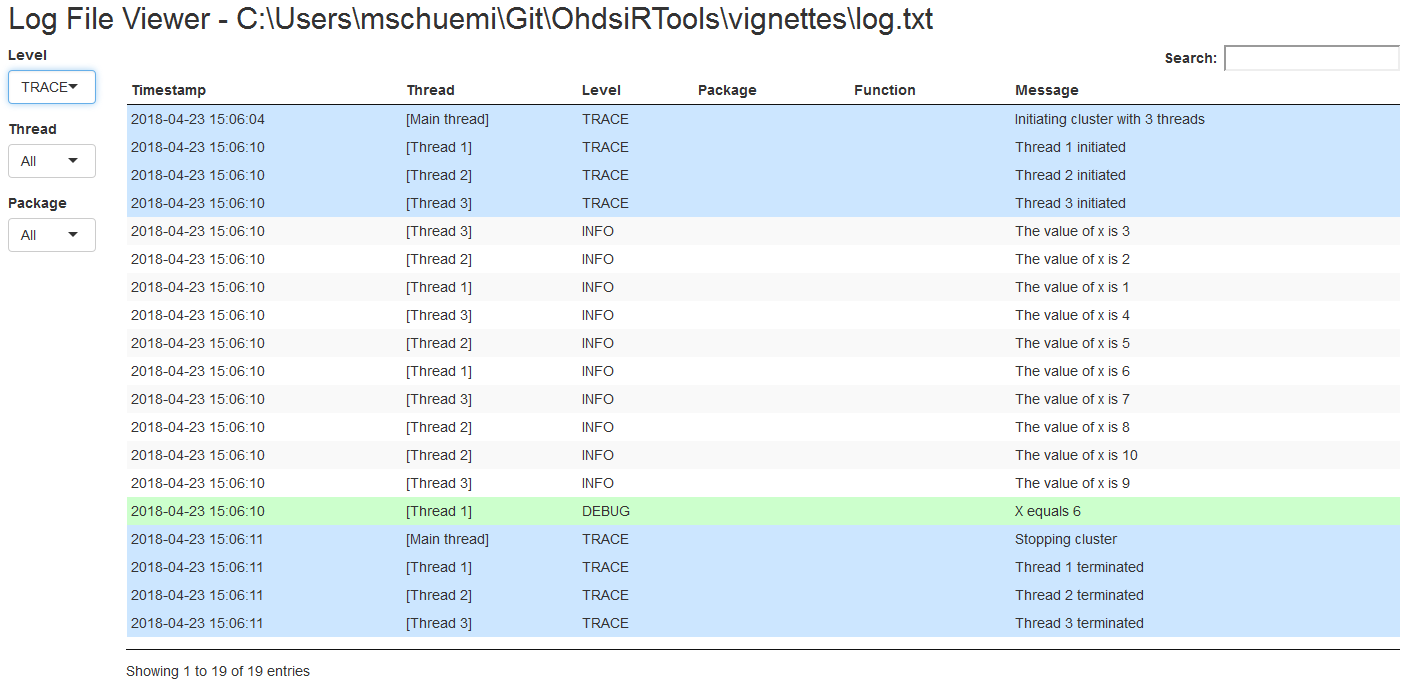
\includegraphics{shinyApp.png}
\caption{Shiny log viewer app}
\end{figure}


\end{document}
